\section{Investigating Trends}\label{sec:results}

SMA crossover-based partitioning of performance observations provides
a systematic method for grouping time-correlated performance events.
Once a divergence region (i.e., a performance trend) has been identified,
more focused statistical analyses can then be applied within the region
to gain insight into the factors that contributed to that trend.  Examples of
contributing factors may include resource utilization, system health, and component performance.
In the following analyses, we separate our 11,986 performance observations into sets of observations that all ran on the same test platform (as described in Table \ref{tab:platform-descriptions}) to characterize the factors that contribute to time-dependent, systemic performance variation across different file systems and architectures.

\subsection{Correlative analysis} \label{sec:results/correlate-mira}

\begin{figure}
    \centering
    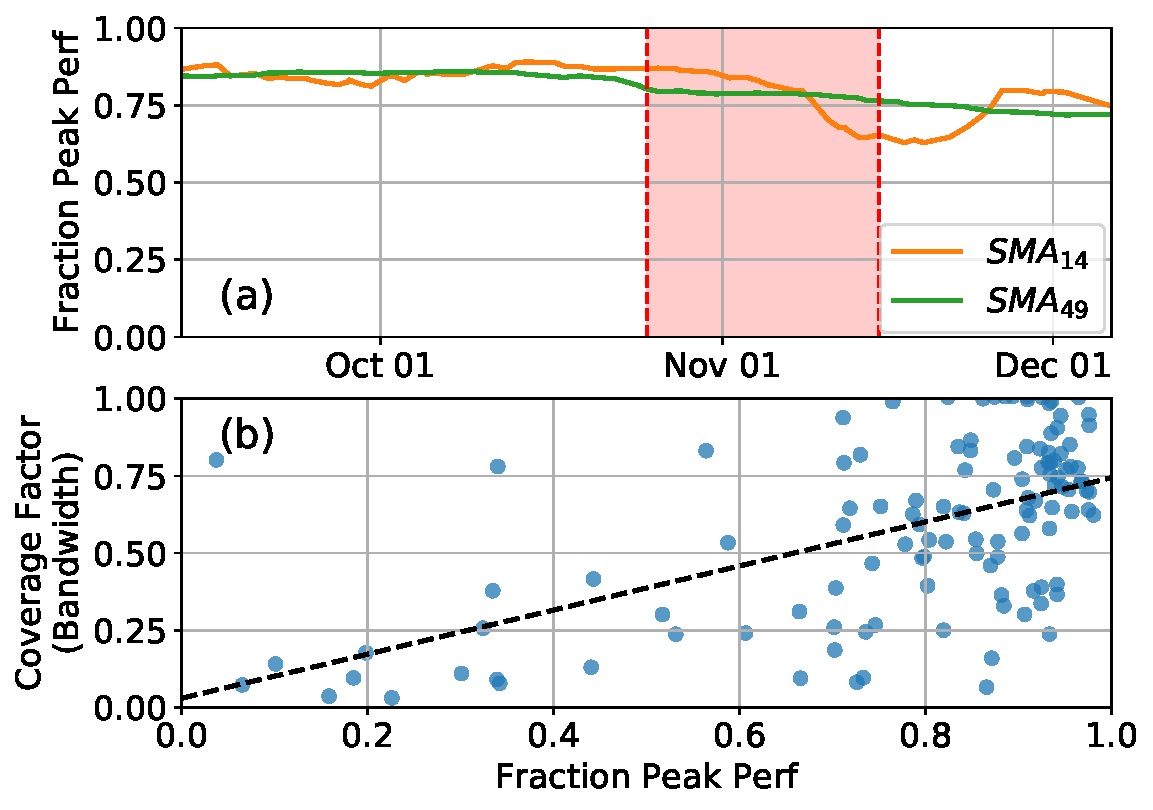
\includegraphics[width=1.0\columnwidth]{mira-correlation-region}
    \vspace{-.35in}
    \caption{Correlation between performance and bandwidth coverage factor in a divergence region on \mira for all I/O motifs combined.
    (a) Divergence region of interest,  corresponding to the same highlighted region shown in Fig. \ref{fig:mira-regions-overview}. (b) Correlation between performance and bandwidth coverage factor in that region.
    Correlation coefficient is $0.507$, and p-value is ${8.71 \times 10^{-9}}$; dashed line in (b) is a linear fit with slope $0.503$ drawn for visual aid.}
    \label{fig:mira-correlation-region}
    % source: sc18-figure6-figure7.ipynb
	\vspace{-.15in}
\end{figure}

We begin our correlative analysis by partitioning a year-long dataset into
divergence regions using the method described in
Section~\ref{sec:features/partitioning}. Using the performance observations across all \mira
\mirafsone workloads as an example, we set ${w_{short} = \textup{two weeks}}$ and ${w_{long}
= \textup{seven weeks}}$ to identify divergence regions and then discard any
regions with fewer than three data points.  Regions with few data points are discarded
for two reasons: (a) intuitively, very short divergence regions occur
when $\textup{SMA}_{short} \approx \textup{SMA}_{long}$ and there is
minimal long-term variation, and (b) statistically, it is impossible
to assert the statistical significance of a correlation with fewer than
three data points.  This yields 32 divergence regions.

We then apply Pearson correlation~\cite{Falk97manyfaces} to the feature vectors within each divergence region to identify the factors that correlate with its
performance trend.
The result of this process is a new feature vector for each divergence region that contains the correlation coefficients between the fraction of peak performance and every other attribute across all observations in that region.
We then use the p-value of each correlation coefficient\footnote{
The p-value of a correlation coefficient is the probability of observing data that would show the same correlation coefficient in the absence of any real relationship between the underlying metrics.
A low p-value indicates that it is extremely unlikely that the calculated correlation coefficient would be observed if the metrics being compared had no real correlation.
As such, p-values represent the statistical significance of a statistical measurement.}
to further down-select the total set of regions to those with extremely high significance
($\textup{p-value} < {1.0 \times 10^{-5}}$).
This threshold yields a total of nine relevant divergence regions on \mira \mirafsone, which are all depicted as shaded extents in Fig. \ref{fig:mira-regions-overview}.
Each of these nine regions exhibits at least moderate correlation ($R$) ranging from 0.507 to 0.884 with the bandwidth coverage factor feature.

Figure~\ref{fig:mira-correlation-region} illustrates the correlation between bandwidth coverage factor and fraction peak performance for a particular divergence region in November 2017 on \mira \mirafsone.
This example shows the lowest correlation ($R = 0.507$) with bandwidth coverage factor of any of the selected regions, and the scatter plot of performance results shows why:
This region contains a cluster of poorly performing probes (${0.2 < \textup{fraction peak perf} < 0.4}$) that ran with a relatively high bandwidth coverage factor.
This region is also the single largest divergence region observed on \mira; a difference of over 20\% between $\textup{SMA}_{short}$ and $\textup{SMA}_{long}$ was observed during this time.
This divergence region example highlights the importance not only of identifying regions and calculating correlations but also of identifying cases in which the analysis indicates the presence of an unknown factor that is not adequately captured by the instrumentation framework.

Despite the unusual region shown in Fig. \ref{fig:mira-correlation-region},
however, the data indicates that the time-dependent performance divergences observed on \mira show either moderate or strong correlation with bandwidth contention.
Additionally, this correlation with performance degradation occurs across
\emph{all} I/O motifs (similar to Fig. \ref{fig:regions-heatmap}a), which
distinguishes it from the motif-specific case discussed in Section
\ref{sec:features/timedependent}.  

When the same Pearson correlation is calculated across the entire collection
of \mira \mirafsone data in the absence of partitioning, the correlation with the bandwidth coverage factor
yields an overall result of $R = 0.483$ and $\textup{p-value} =
2.25\times 10^{-88}$.  
Thus, significantly stronger correlations can be found by focusing analysis on algorithmically identified regions of
interest in the data.

\subsection{Survey of divergence regions} \label{sec:results/correlate-all}

\begin{figure}
    \centering
    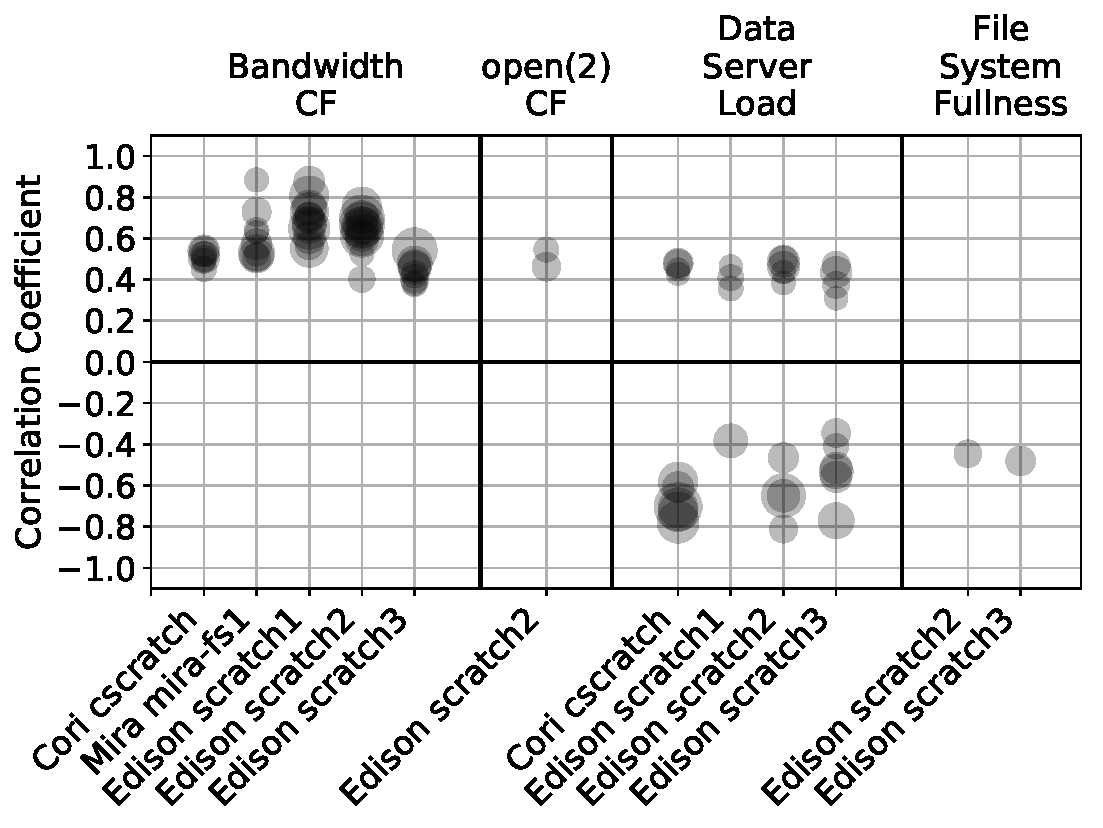
\includegraphics[width=1.0\columnwidth]{trend-correlations}
    \vspace{-.35in}
    \caption{Correlations discovered between fraction peak performance and all other attributes measured during job execution.
    Each circle represents the correlation coefficient over a single trend region, and its diameter is proportional to $-\log_{10}(\textup{p-value}$).
    CF denotes coverage factor.}
    \label{fig:trend-correlations}
    \vspace{-.15in}
    % source: sc18-figure8-figure9.ipynb
\end{figure}

Next we apply the same correlation analysis to the other test platforms in our study, again  keeping only those correlations with an extremely high significance ($\textup{p-value} < {1.0 \times 10^{-5}}$). The results of this analysis are shown in Fig. \ref{fig:trend-correlations}.
As was found with Mira in Section \ref{sec:results/correlate-mira}, a moderate to strong correlation exists between I/O performance and the bandwidth coverage factor on the Lustre file systems of \cori and \edison.
Although bandwidth contention resulting in performance loss is intuitive at the scale of a single performance transient, the fact that these correlations were found over longer-term divergence regions indicates that bandwidth contention from sustained, I/O-intensive workloads often accompanies sustained performance losses.
This fact is particularly relevant to the increasing fraction of experimental and observational data that is being processed on modern HPC platforms; as the volume of data being continually streamed from large-scale scientific instruments increases, the effects of sustained bandwidth contention are likely to become increasingly prominent.

\begin{figure}
    \centering
    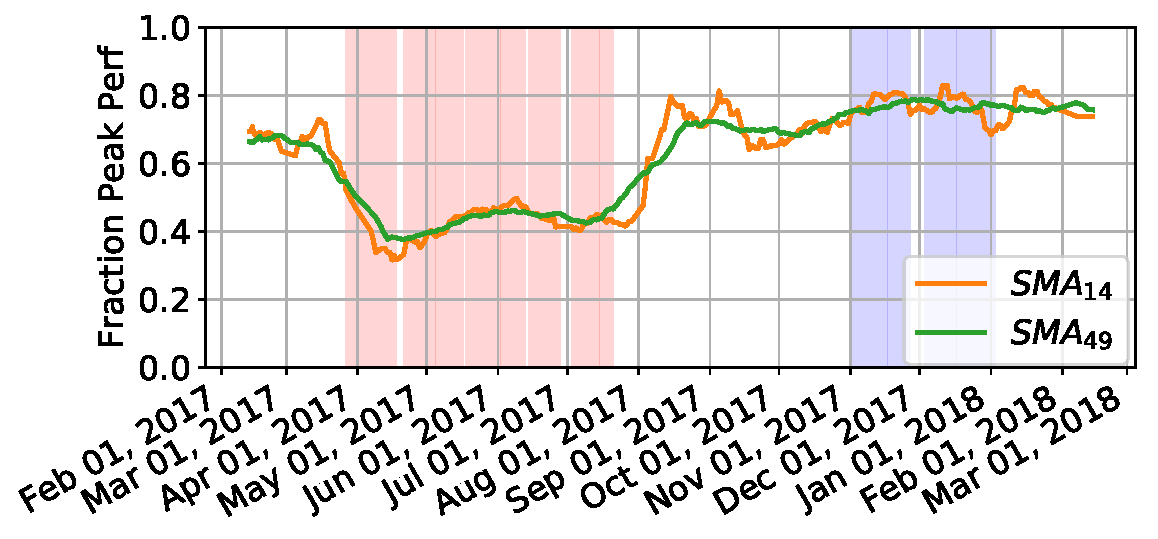
\includegraphics[width=1.0\columnwidth]{cscratch-bimodal-fsaveosscpu}
    \vspace{-.35in}
    \caption{Regions of negative correlation (red) and positive correlation (blue) between fraction peak performance and data server load during divergence regions identified on \cori.
    SMAs for \cori's HACC write workload are also shown to illustrate the coincidence of a long-term performance issue with the direction of correlation.}
    \label{fig:cscratch-bimodal-fsaveosscpu}
    % source: sc18-figure8-figure9.ipynb
    \vspace{-.15in}
\end{figure}

Another noteworthy feature that this method reveals is the bimodality of correlation between performance and the CPU load of the file system data servers (``Data Server Load'' in Fig. \ref{fig:trend-correlations}) on the Lustre-based test platforms.
A time-resolved view of the regions where performance correlates with data server CPU loads (Fig. \ref{fig:cscratch-bimodal-fsaveosscpu}) reveals that the bimodality of the correlation matches the biomodality observed in the HACC write workload on the affected storage systems.
During the long-term performance regression discussed in Section \ref{sec:features/timedependent}, high CPU load on the Lustre data servers coincided with low I/O performance probe performance.
Once performance was restored on August 10, the relationship reversed, and high CPU load correlated favorably with performance.

The positive correlation between performance and CPU load is consistent with the data servers using CPUs to service incoming I/O requests, whereas the negative correlation indicates that another CPU load (as may result from a software bug) was present and competed with the servers' ability to use CPU to service I/O requests.
From these results we conclude that not only does baseline I/O performance vary with time but also the nature and magnitude of how different attributes correlate with I/O performance  change over time.
Had this correlation analysis been performed without partitioning over divergence regions, the regions of positive and negative correlation would have obfuscated each other in the net result.

The remaining two attributes that were found to correlate with performance
are file system fullness and \texttt{open(2)} coverage factor (a
measure of metadata resource contention).  The two instances of file
system fullness correlating negatively with performance are clear
and were corroborated with independent observations from facilities
staff.  These two regions encapsulate periods when their respective
file systems approached 90\% fullness for a period of several days.
The observed loss of performance is consistent with Lustre's known
susceptibility to significant performance degradation as OSTs approach
90\% fullness~\cite{oral2014best,Lockwood2017}.

The correlation with
\texttt{open(2)} coverage factor is intuitive because this metric acts as a
proxy for metadata contention.  
One of these divergence regions was found to overlap with an unusually extensive, long-running multiday purge of the \edison \scratchtwo file system.
However,  at this time the cause of the other correlated divergence region is unclear. (We will continue to investigate.)
% The above statement is not very satisfying, but we don't have time to do more detailed analysis.  The regions are:
% coverage_factor_opens 2017-03-29 19:11:51 - 2017-04-15 19:13:37 (71 points)
% coverage_factor_opens 2017-11-26 18:26:41 - 2017-12-13 20:03:11 (141 points)


\subsection{Transient performance loss} \label{sec:results/shortterm}

\begin{figure}
    \centering
    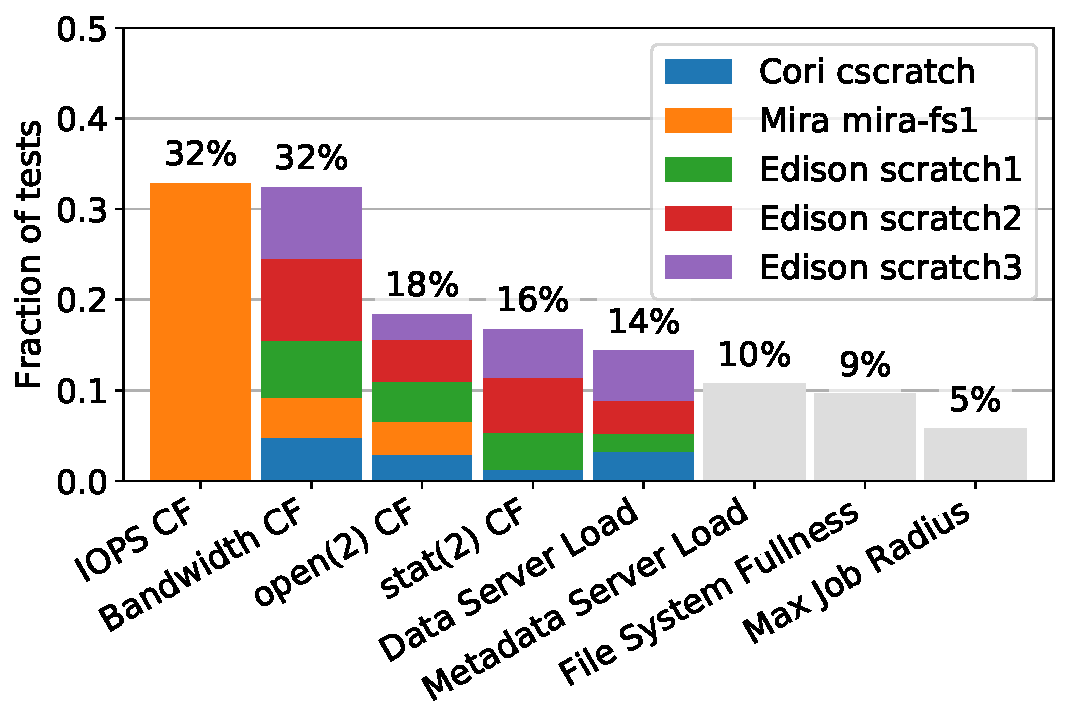
\includegraphics[width=1.0\columnwidth]{contributors-bad-by-system-grey}
    \vspace{-.35in}
    \caption{Attributes that correlated with poor I/O performance across all file systems and benchmarks tested, normalized to the number of probes during which each attribute was measured.
    \mira was the only system for which IOPS coverage factor was measured.
    Gray bars are attributes whose rate of classification were not statistically significant.
    Percentages do not add up to 100\% because multiple attributes are often classified as contributors for a single anomalous observation.
    }
    \label{fig:contributors-bad-by-system}
    % source: sc18-figure10.ipynb
    \vspace{-.15in}
\end{figure}

In addition to characterizing long-term performance issues, it is  advantageous to determine the reasons why I/O performance is severely degraded for one and only one day in an otherwise unremarkable period of time.
Such performance losses, indicated by isolated dark blocks in Fig. \ref{fig:regions-heatmap}, may  be observed in only one of the I/O performance probes issued on a given day and suggest a very short-lived issue that disappeared over the course of one or two of the eight daily probes.
The lack of a consistent performance trend surrounding these transients makes them difficult to correlate with other metrics as was done in the preceding section, necessitating a different approach to characterizing them.

To address this need, we apply the same strategy of partitioning performance observations into divergence regions and then performing statistical analysis within each region.
To identify individual performance anomalies in a divergence region and classify the factors which contributed to them, we apply the following binary classification method.

\begin{enumerate}[leftmargin=*]

\item We examine the feature vector for every observation in the divergence region, and for each attribute $a$ we determine the observation where that attribute's measured value was at its lowest, $\min(a)$.

\item We then define the \emph{anomalous observation} for the divergence region as the observation whose feature vector contains $\min(a)$ for fraction peak performance.
Since divergence regions contain observations of similar performance by definition, this anomalous observation is truly anomalous---it is differentiated from the long-term performance trends described in Sec.~\ref{sec:features} as well as the ones within its own divergence region.

\item We then determine which other $\min(a)$ values also fall in this anomalous observation's feature vector, and we classify those attributes as contributors to the anomalous observation's performance.

\end{enumerate}

Qualitatively, this process codifies the conjecture that if I/O performance is anomalous on a specific day, the other measured attributes that were also anomalous at that time are what contributed to that behavior.
Quantitatively, this simple classification scheme allows us to identify relationships and define the statistical significance of each classification for individual anomalous observations using p-values.\footnote{
The p-value is the probability of making a positive classification in the absence of an underlying relationship or, equivalently, the probability of positively classifying a random value.
Since there is only one $\min(a)$ in each region of $N$ observations, the p-value for our classifications is thus $\frac{1}{N}.$}

The result of this process is zero or more attributes being positively classified as contributors to anomalous performance.
For example, if the lowest values of the bandwidth coverage factor and IOPS coverage factor attributes occur in the same feature vector as the lowest value for performance, we classify both bandwidth and IOPS coverage factors as contributors to that anomalous observation's performance.

To apply this method, we first group observations into sets of data by the test platform on which they ran.
These sets are then further subdivided according to I/O motif and read/write mode of the probe to classify anomalies at full temporal resolution and motif-level granularity.
The net result are $5 \times 4 \times 2 = 40$ sets of data, each representing a unique combination of test platform ($5 \times$, as listed in Table \ref{tab:platform-descriptions}), I/O motif ($4 \times$, per Table \ref{tab:benchmark-motifs}), and whether the probe was reading or writing ($2 \times$).
Schematically, each horizontal row in Fig. \ref{fig:summary-heatmap} represents a single set.
For each set of observations, SMAs are calculated, crossover points are defined, and the set is partitioned into a set of divergence regions.

This partitioning results in 1,146 divergence regions across 40 sets of observations.
For each such region, we then apply the aforementioned binary classification to identify anomalous observations and classify attributes that affected performance.
All statistically insignificant classifications ($\textup{p-value} > 0.10$) are discarded, in order to eliminate divergence regions that are too small to make any meaningful classifications. The final products are 
490 anomalous observations, 410 (84\%) of which have at least one positively classified attribute.

Not every observation's feature vector has every feature defined as a result of some monitoring components being offline at the time of a test.
To avoid biasing our results away from those attributes that were measured for only a subset of observations, we express the importance of each attribute as the number anomalous observations where it was positively classified divided by the total number of observations where it was measured.
Figure \ref{fig:contributors-bad-by-system} enumerates the attributes that were positively classified the most times.

As with the longer-term performance divergence characterized in Section \ref{sec:results/correlate-all}, high contention for bandwidth also coincides with short-term performance transients.
In contrast, contention for IOPS is positively classified in a significant fraction of anomalous observations despite its not arising as a factor in longer-term performance divergence.
This contrast suggests that IOPS contention  becomes a significant contributor to performance degradation only in short-term transients.
Conversely, we conclude that periods of high IOPS contention do not last long enough to be implicated in long-term performance degradation on production file systems, whereas the same is not true of bandwidth contention. These are two distinct forms of performance variation that
require unique investigation techniques to uncover.

We also observe the coincidence of anomalous observations and anomalous metadata coverage factors and CPU load on data servers to a less significant degree.
This is consistent with the moderate correlations shown in Figure~\ref{fig:trend-correlations}.
Unlike the correlative analysis, however, this transient analysis shows that metadata contention impacts individual jobs on every test platform, and it is observed at much higher frequency on short time scales.
This indicates that, like IOPS contention, metadata contention is much more likely to coincide with transient performance loss than a long-term performance divergence.

Metadata server CPU load, file system fullness, and maximum job radius were also classified in some anomalous observations.
However, the low number of anomalous observations in which they appeared calls into question the statistical significance of these three findings.
To address this result, we calculate the p-values (the probability of observing the same number of classifications in the absence of a true underlying relationship) for each metric using binomial tests.\footnote{
We use one-tailed binomial tests with the number of positive classifications ($k$) and total observations ($n$) for each metric.
The fact that our dataset was filtered to include only  regions with ${\textup{p-value} < 0.10}$ allows us to use 0.10 as a conservative value for the probability of success ($p$).}

These significance tests reveal that the number of times metadata server load, file system fullness, and maximum job radius were classified is statistically insignificant.
Whereas the leftmost five attributes in Fig. \ref{fig:contributors-bad-by-system} all have p-values of ${5 \times 10^{-5}}$ or lower, the insignificant metrics are 0.15 or higher.
Qualitatively, these negative findings are not unreasonable; for example, file system fullness is most often a degenerative, long-term health problem, as was identified in Section \ref{sec:results/correlate-all} and prior work~\cite{oral2014best,Lockwood2017}.
Thus, while it may coincide with transient anomalies, it is unlikely to be the sole contributor to poor performance for a transient anomaly.

The classification and analysis described here demonstrate that one can apply statistical analysis to fine-grained divergence regions and still obtain statistically significant insight into the causes of transient performance degradation.
While we chose a  simple binary classification criterion based on $\min(a)$, this process could be applied using any classification methodology that identifies relationships between feature vectors and quantifies the associated statistical significance.
